%% Copyright 2018 H.\ Rabus
%
% This work may be distributed and/or modified under the
% conditions of the LaTeX Project Public License, either version 1.3
% of this license or (at your option) any later version.
% The latest version of this license is in
%   http://www.latex-project.org/lppl.txt
% and version 1.3 or later is part of all distributions of LaTeX
% version 2005/12/01 or later.
%
% This work has the LPPL maintenance status `author-maintained'.
%
% This work consists of the file texbsp.tex
%

\documentclass[smallheadings]{scrartcl}

%%% GENERAL PACKAGES %%%%%%%%%%%%%%%%%%%%%%%%%%%%%%%%%%%%%%%%%%%%%%%%%%%%%%%%%%
% inputenc allows the usage of non-ascii characters in the LaTeX source code
\usepackage[utf8]{inputenc}
\usepackage{graphicx} 
\usepackage{float}
%\graphicspath{ {/u/hnatiuka/Praktikum/PPI/} }



% title of the document
\title{Bericht zu Serie 3}
% optional subtitle
%\subtitle{Draft from~\today}
% information about the author
\author{%
  Arsen Hnatiuk,\\%
  Max Huneshagen 
}
\date{\today} 


%%% LANGUAGE %%%%%%%%%%%%%%%%%%%%%%%%%%%%%%%%%%%%%%%%%%%%%%%%%%%%%%%%%%%%%%%%%%
% babel provides hyphenation patterns and translations of keywords like 'table
% of contents'
\usepackage[ngerman]{babel}

%%% HYPERLINKS %%%%%%%%%%%%%%%%%%%%%%%%%%%%%%%%%%%%%%%%%%%%%%%%%%%%%%%%%%%%%%%%
% automatic generation of hyperlinks for references and URIs
\usepackage{hyperref}

%%% MATH %%%%%%%%%%%%%%%%%%%%%%%%%%%%%%%%%%%%%%%%%%%%%%%%%%%%%%%%%%%%%%%%%%%%%%
% amsmath provides commands for type-setting mathematical formulas
\usepackage{amsmath}
\numberwithin{equation}{section}
% amssymb provides additional symbols
\usepackage{amssymb}
% HINT
% Use http://detexify.kirelabs.org/classify.html to find unknown symbols!

%%% COLORS %%%%%%%%%%%%%%%%%%%%%%%%%%%%%%%%%%%%%%%%%%%%%%%%%%%%%%%%%%%%%%%%%%%%
% define own colors and use colored text
\usepackage[pdftex,svgnames,hyperref]{xcolor}

%%% Code Listings %%%%%%%%%%%%%%%%
% provides commands for including code (python, latex, ...)
\usepackage{listings}
\definecolor{keywords}{RGB}{255,0,90}
\definecolor{comments}{RGB}{0,0,113}
\definecolor{red}{RGB}{160,0,0}
\definecolor{green}{RGB}{0,150,0}
\lstset{language=Python, 
        basicstyle=\ttfamily\small, 
        keywordstyle=\color{keywords},
        commentstyle=\color{comments},
        stringstyle=\color{red},
        showstringspaces=false,
        identifierstyle=\color{green},
        }


\usepackage{paralist}
\usepackage{nicefrac}
% setting the font style for input und returns in description items
\newcommand{\initem}[2]{\item[\hspace{0.5em} {\normalfont\ttfamily{#1}} {\normalfont\itshape{(#2)}}]}
\newcommand{\outitem}[1]{\item[\hspace{0.5em} \normalfont\itshape{(#1)}]}
\newcommand{\bfpara}[1]{
	
	\noindent \textbf{#1:}\,}


\begin{document}

% generating the title page
\maketitle
% generating the table of contents (requires to run pdflatex twice!)
\tableofcontents
\bigskip

\hrule
\hrule

%%% BEGIN OF CONTENT %%%%%%%%%%%%%%%%%%%%%%%%%%%%%%%%%%%%%%%%%%%%%%%%%%%%%%%%%%

\section{Einleitung}

\subsection{Laplace Gleichung}
Die in dieser Serie implementierten Programme ermöglichen die Lösung des in Serie 2 betrachteten Gleichungssystems
\begin{align}
	A^{(d)}\hat{u} = b
	\label{eq:glc}
\end{align}
wobei $A^{(d)}$ eine Bandmatrix der Dimension $d$ und $\hat{u}$ eine Approximation der Lösung der Laplace Gleichung ist. $b$ ist der Vektor der Randbedingungen und der Werte der in der Laplace Gleichung gegebenen Funktion $f$ auf den in Serie 2 ausgewählten Punkten. Da alle Randbedingungen in dieser Serie $0$ sind, ist $b$ einfach der Vektor der $f_i := f(x_i)$ für die ausgewählten $x_i$. 

Die Lösung dieses Systems erfolgt durch die LU-Zerlegung der $A^{(d)}$ Matrix. Wir können also $TA^{(d)}=LU$ für eine Permutationsmatrix $P$, eine unipotente untere Dreiecksmatrix $L$ und eine invertierbare obere Dreiecksmatrix $U$ schreiben. Dann lässt sich die Gleichung \ref{eq:glc} so darstellen:
\begin{align}
	T^tLU\hat{u}=b
	\label{eq:lu}
\end{align}
Man gewinnt die Werte von $\hat{u}$, indem man mittels Rückwärtssubstitution die Gleichung 
\begin{align}
	T^tLz=b
	\label{eq:lu1}
\end{align}
für ein $z\in \mathbb{R}^{(n-1)^d}$ löst. Dies ist möglich, weil $L$ eine Dreiecksmatrix mit Einsen auf der Hauptdiagonale ist. Die Werte von $\hat{u}$ rechnet man durch Rückwärtssubstitution in der Gleichung \eqref{eq:lu2} aus. Dies ist möglich, weil alle Hauptdiagonaleinträge von $R$ nach Numerische Lineare Algebra ungleich $0$ sind (dies sind die sogenannten Pivotelemente).
\begin{align}
	R\hat{u}=z
	\label{eq:lu2}
\end{align}
Wenn man die Gleichungen \eqref{eq:lu1} und \eqref{eq:lu2} zusammensetzt, so erhält man \eqref{eq:lu}.

\subsection{Hilbert-Matrizen}
Unsere Programme ermöglichen auch die Arbeit mit Hilbert-Matrizen. Diese dienen als Beispiel schlecht konditionierter Matrizen und sind wie folgt definiert:
\begin{align}
	H_m &:= (a_{ij})_{1\le i, j \le m} \in \mathbb{R}^{m\times m}, 	\\
	a_{ij} &:= \frac{1}{i+j-1} \label{eq:hb1}
\end{align}
Das Inverse einer Hilbert-Matrix ist wie folgt definiert:
\begin{align}
	H_m^{-1}& := (b_{ij})_{1\le i, j \le m} \in \mathbb{R}^{m\times m},	\\
	b_{ij} := \frac{(-1)^{i+j}}{i+j-1}\cdot &\frac{(m+i-1)!}{(i-1)!^2(m-i)!}\cdot \frac{(m+j-1)!}{(j-1)!^2(m-j)!}
\end{align}

Aus der numerischen linearen Algebra wissen wir, dass für die Kondition $\kappa$ einer Matrix $A$ gilt
\begin{align}
	\kappa(A)=\|A\|\cdot \|A^{-1}\|
\end{align}
Wenn wir die Spaltensummennorm $\|\cdot \|_{\infty}$ benutzen, ist die hohe Kondition einer Hilbert-Matrix leicht zu sehen. Aus \ref{eq:hb1}  sieht man, dass die erste Spalte von $H_m$ die höchste Spaltensumme hat, und es gilt
\begin{align}
	\|H_m\|_{\infty}=\sum_{i=1}^{m}\frac{1}{i}
\end{align}
Diese Reihe divergiert. Die Einträge von $H_m^{-1}$ sind dabei sehr groß. Schon für $i=j=1$ gilt $b_{ij} = m^2$, also die Norm von dieser Matrix wächst mindestens quadratisch. Folglich ist die Kondition $\kappa(H_m)\gg1$ für $m>1$.

\section{Theorie}

\subsection{Fehlerabschätzung mit Hilfe der Kondition}

Nach Bemerkung~4.4 des Skriptes \textit{Numerische Lineare Algebra} entspricht die Kondition $\kappa(A)$ einer Matrix $A$ der relativen Kondition des linearen Gleichungssystems $f(x)=b \iff Ax=b$. 

\section{Experimente}

Gemäß Aufgabe~3.6 der Aufgabenstellung wurde die Kondition der Hilbertmatrix $H_m$ in Abhängigkeit der Matrixgröße $m$ experimentell untersucht und graphisch dargestellt. Ebenso wurde das Gleichungssystem 
\begin{align}
H_mx^{(i)}=e_i
\label{eq:hil_lgs}
\end{align}
für $m=2^k$, $k=0,1,2,\dots$ numerisch unter Ausnutzung der $L$-$U$-Zerlegung (s.~Schnittstellendoku) gelöst. Die aus den numerischen Verfahren gewonnene Lösung $\tilde{x}^{(i)}$ wurde mit der exakten Lösung $x^{(i)}$ verglichen. Letztere ergibt sich aus \eqref{eq:hil_lgs} als die $i$-te Spalte der inversen Hilbert-Matrix:
\begin{align}
x^{(i)}=H_m^{-1}e_i\equiv(\text{$i$-te Spalte von }H_m^{-1}).
\end{align}
Die beiden Vektoren wurden anhand der Größe
\begin{align*}
\max\limits_{i=1,\dots,m}\|\tilde{x}^{(i)}-x^{(i)}\|_\infty
\end{align*}
verglichen. Das Ergebnis ist in Abb.~\ref{fig:hil_kond_fehl}
dargestellt.

\begin{figure}[H]
\centering
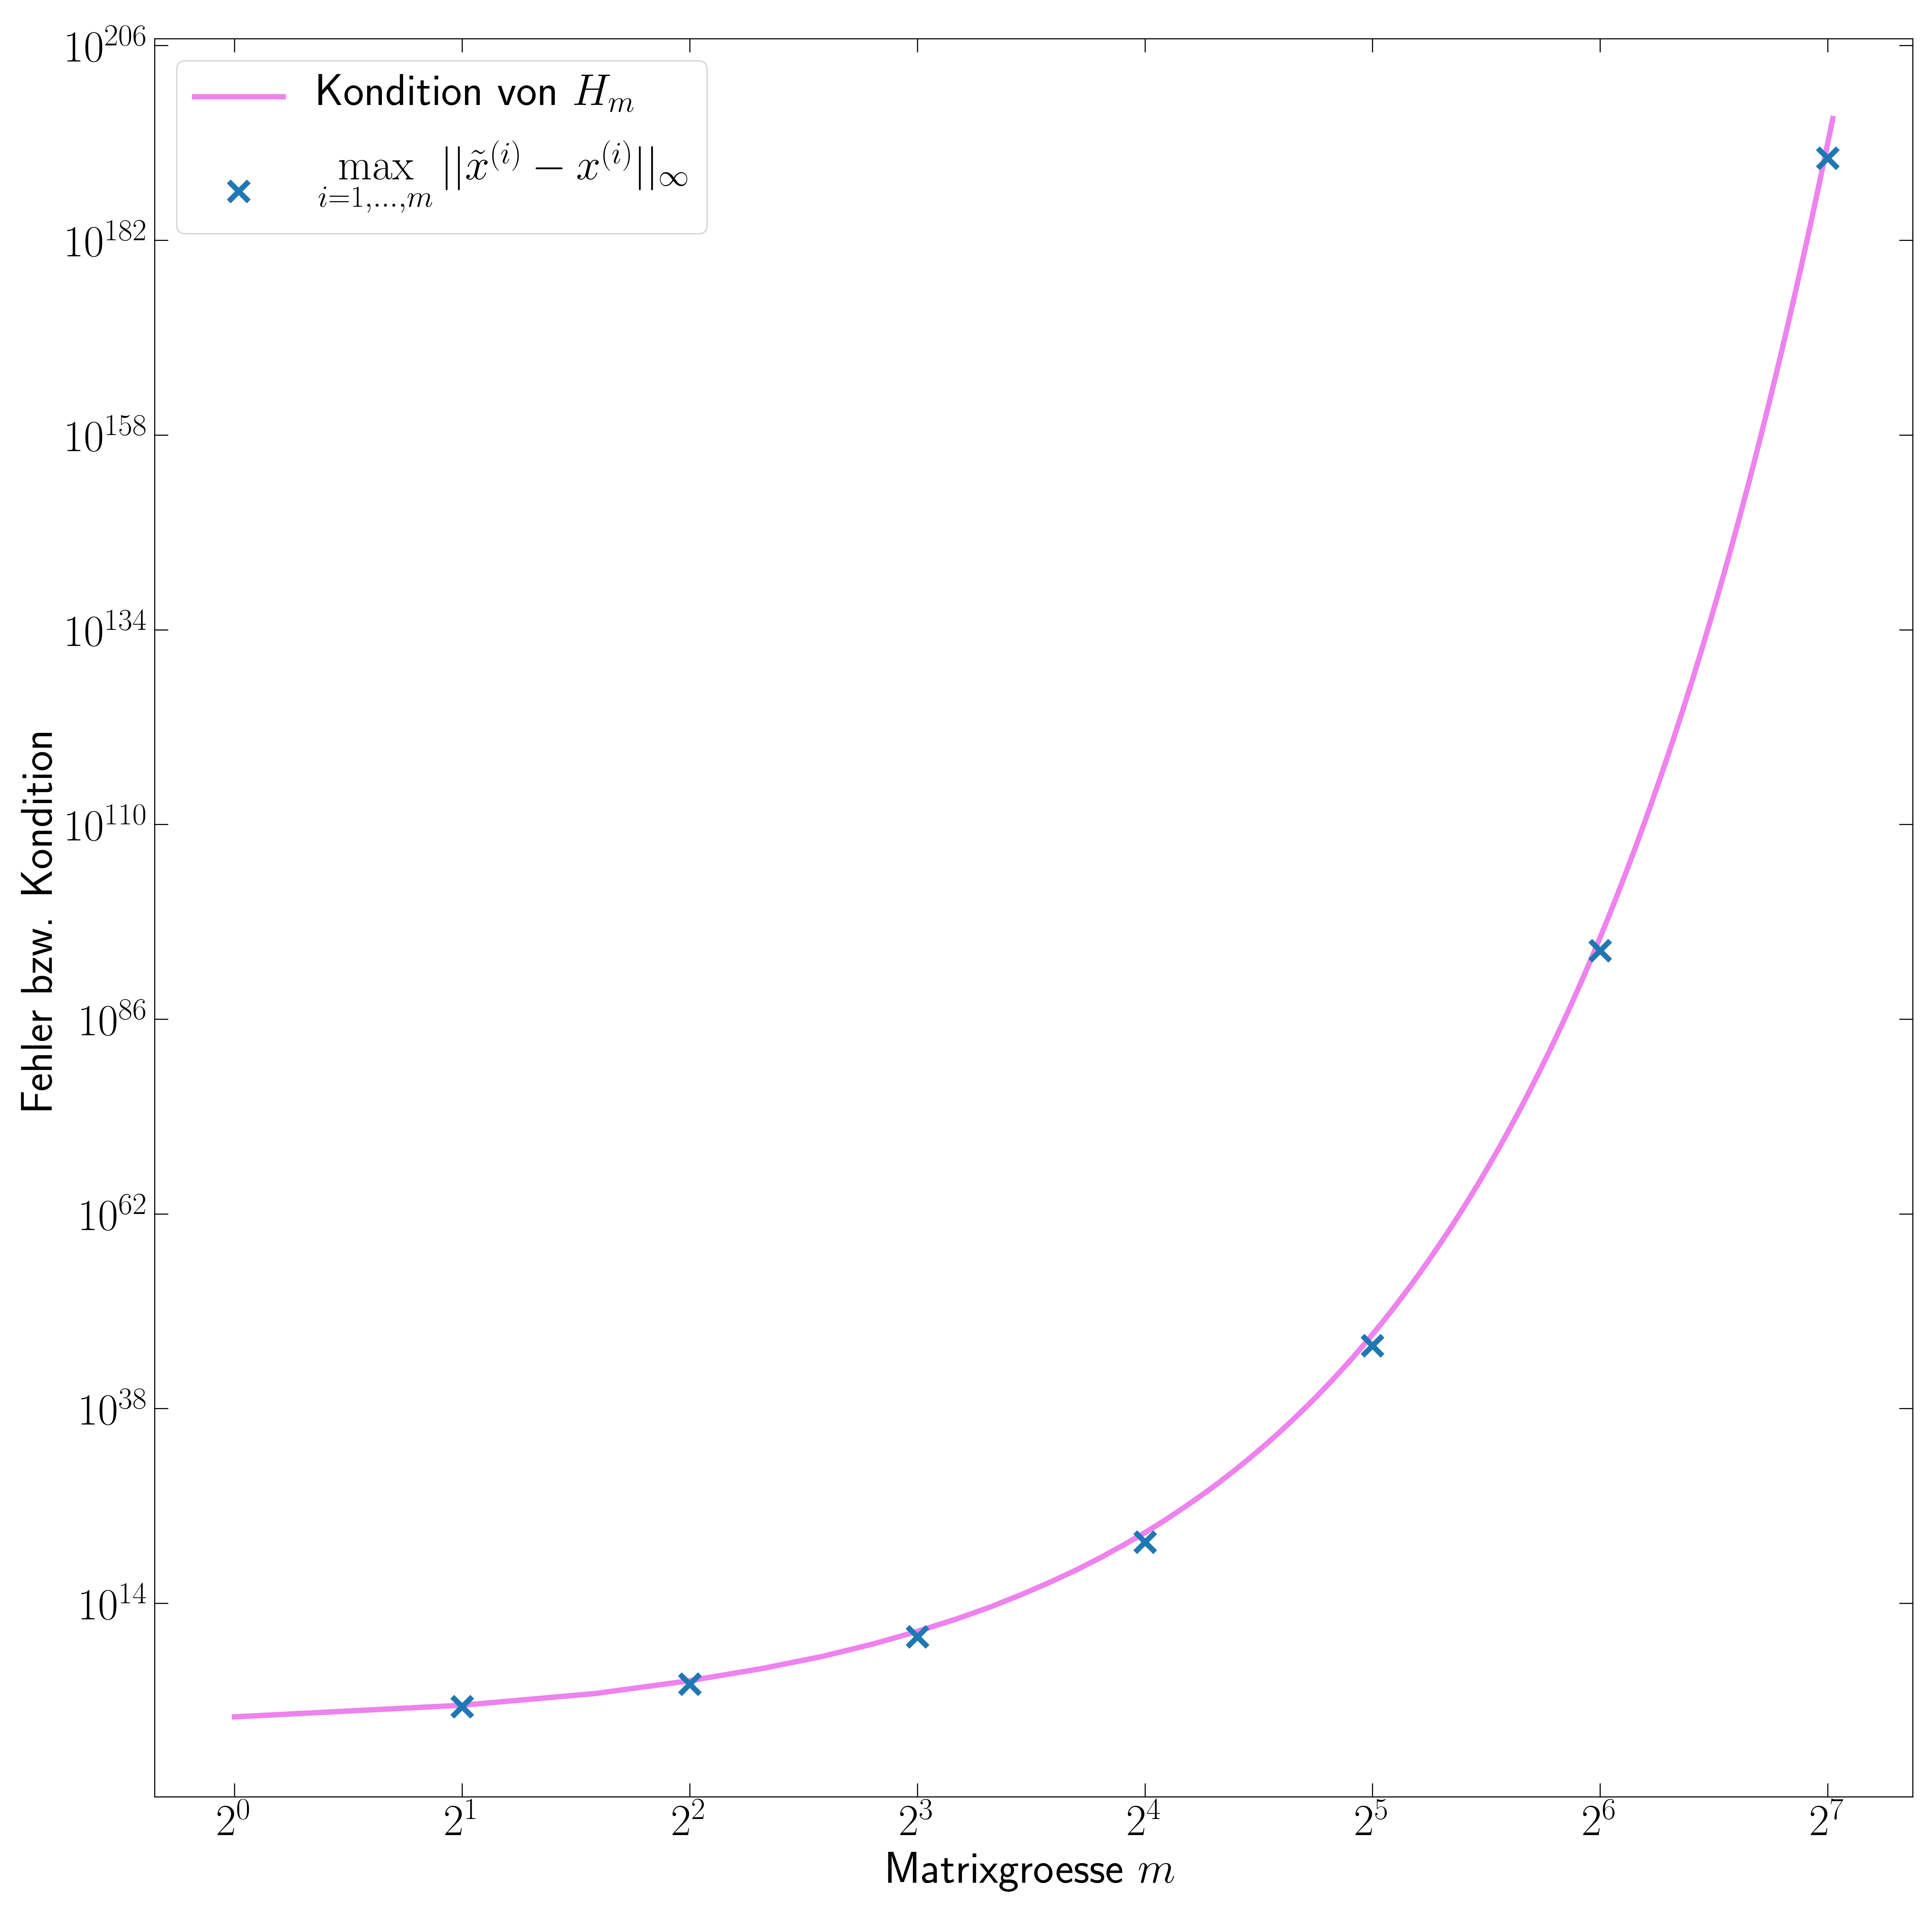
\includegraphics[width=.8\textwidth]{Bericht/Bilder/hil_kond_fehl}
\label{fig:hil_kond_fehl}
\caption{Fehler der numerischen Lösung von \eqref{eq:hil_lgs} und Kondition von $H_m$ in Abhängigkeit von der Matrixgröße $m$.}
\end{figure}

Man erkennt ein starkes Ansteigen der Kondition von $H_m$ mit $m$. $\kappa(H_m)(m)$ ist in der logarithmischen Darstellung im betrachteten Bereich monoton wachsend und konvex, wächst also schneller als jede endliche Potenz von $m$. Der Wert von $\max\|\tilde{x}^{(i)}-x^{(i)}\|_\infty$ ist für die betrachteten $m$ durch $\kappa(H_m)$ beschränkt.

\section{Zusammenfassung}


\begin{thebibliography}{9}
\bibitem{wiki} Kein Autor, Aufgerufen am 22.11.2018, \textit{Sparse Matrix}. 
\url{https://en.wikipedia.org/wiki/Sparse_matrix}
\end{thebibliography}


%%% END OF DOCUMENT %%%%%%%%%%%%%%%%%%%%%%%%%%%%%%%%%%%%%%%%%%%%%%%%%%%%%%%%%%%
\end{document}
